\chapter{User's Manual} \label{ch:manual}

This chapter will describe the usage and features of the \SB in detail and serve as a user's manual. 
\autoref{sec:manual-overview} will give an overview of the IEC editor and the process of creating the IEC project. 
\autoref{sec:manual-sdg} will cover the steps needed to use the \SB. A detailed description of the \SB features will be 
given in \autoref{sec:manual-features}. Finally \autoref{sec:manual-usecases} will cover each use case and include 
examples of problems that might be solved.


\section{Overview} \label{sec:manual-overview}

After first installing the \SB plugins and opening the \emph{\SB} perspective, the Eclipse workbench should look like 
\autoref{fig:manual-perspective}. On the left and right are the standard Eclipse Project Explorer and Outline views, 
respectively. On the bottom is the new \SB view, below the Project Explorer is the Instance Hierarchy view. Those two 
views can be opened in any other perspective using the \emph{Show View} dialog (Alt+Shift+Q, Q by default) as shown in 
\autoref{fig:manual-open_views}.

\begin{figure}[hp]
  \centering
    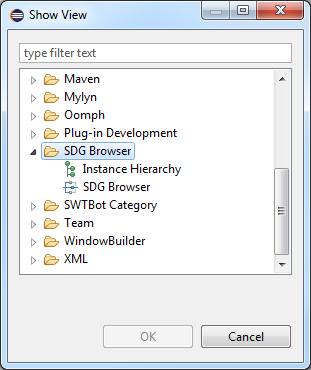
\includegraphics[scale=0.55]{bilder/manual-open_views}
  \caption{Entries in the \emph{Show View} dialog for the \SB views}
  \label{fig:manual-open_views}
\end{figure}

\begin{figure}[htp]
  \centering
    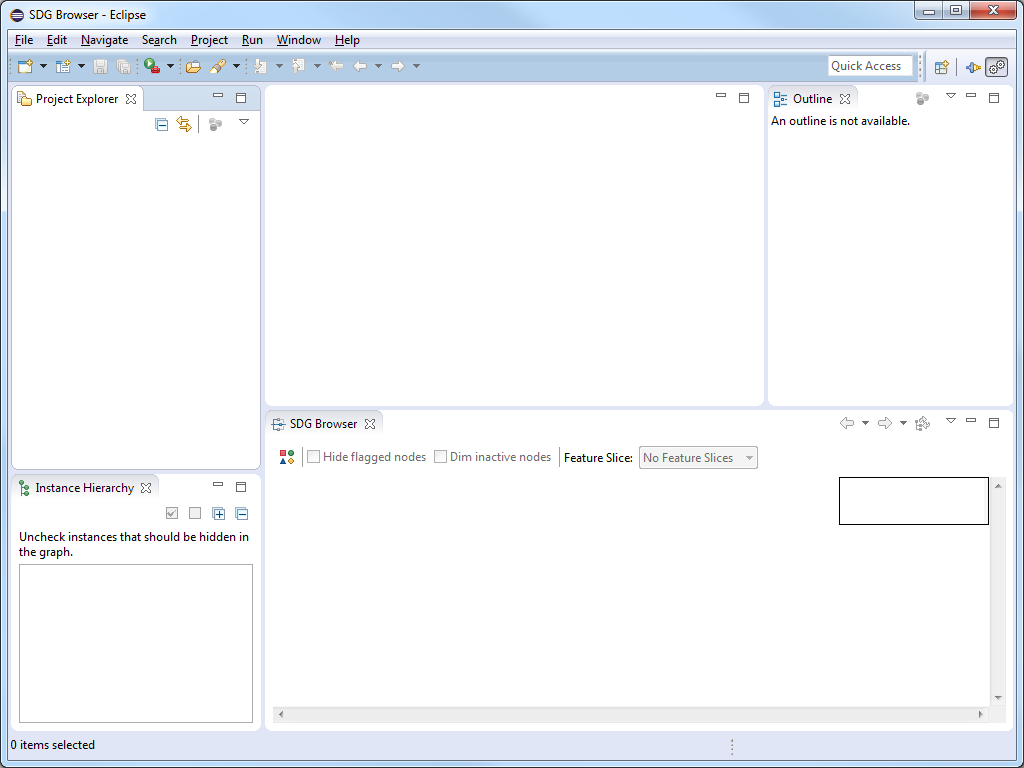
\includegraphics[width=\textwidth]{bilder/manual-perspective}
  \caption{Default layout of the \emph{\SB} perspective}
  \label{fig:manual-perspective}
\end{figure}

In order to use the \SB with IEC source code, you first need to build it in IecEdit and import it as an Eclipse IEC 
Project. A project also needs to be rebuilt in IecEdit whenever it is moved to a different location.

\begin{enumerate}
  \item Create a new Eclipse project and select \emph{IEC Project} from the IEC category (see 
  \autoref{fig:manual-new_project1}).
  
  \item On the next page, enter a name for the project and select the location of the IEC project files 
  (\autoref{fig:manual-new_project2}). This is the location where the Eclipse project file will be created, the IEC 
  source code may be located there or in any subdirectory.
  
  \item In case you have a standard project layout with HMI, the default source code locations may be used 
  (\texttt{/Source/IMM/ieccontrol} and \texttt{/Source/view/viewKVS} for IEC and view code, respectively). Otherwise, 
  uncheck the checkbox and specify the paths (relative to the project location selected earlier). If you don't have an 
  HMI, leave that text box empty.
\end{enumerate}

\begin{figure}[hp]
  \centering
    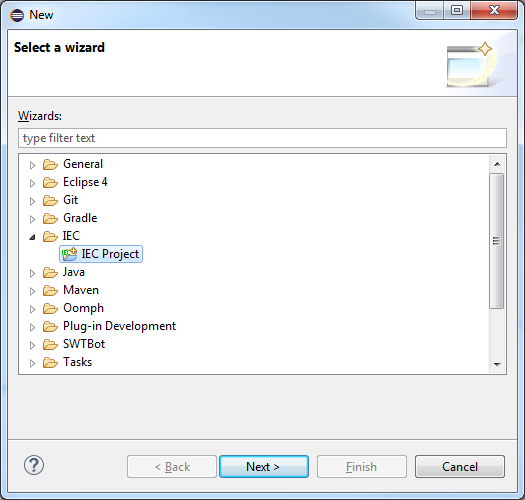
\includegraphics[scale=0.55]{bilder/manual-new_project1}
  \caption{Create a new IEC project\ldots}
  \label{fig:manual-new_project1}
\end{figure}

\begin{figure}[hp]
\centering
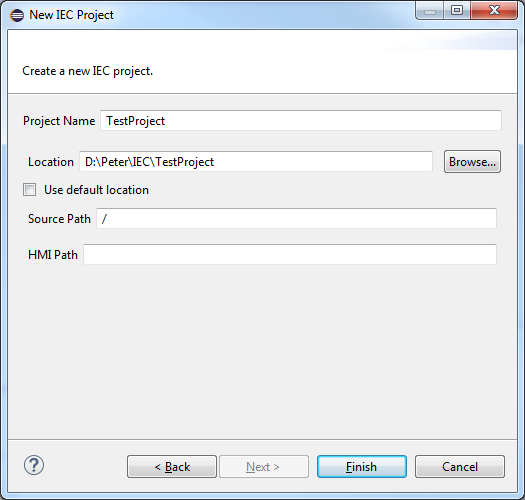
\includegraphics[scale=0.55]{bilder/manual-new_project2}
\caption{\ldots{}and specify the source code location}
\label{fig:manual-new_project2}
\end{figure}

After the project has been created, the Project Explorer will show all files and folders under the project directory, 
with some exceptions. Files recognized by any Eclipse editor can be opened directly, including IEC source files. Note, 
however, that the IEC editor as it's currently implemented doesn't allow editing. This is so files containing Keba's 
proprietary representation of the source code (the so called \emph{UFF code}), in addition to the textual IEC code, 
don't get corrupted.

By default, IEC binaries and files related to Keba's IecEdit will not be shown in the Project Explorer. This may be 
changed by disabling the respective filters in the Project Explorer (via the \emph{Customize View...}\ menu item).

\autoref{fig:manual-editor} shows an IEC file opened in the Eclipse editor. Note the file outline on the right hand 
side. The IEC editor shows only the textual IEC code, the UFF code is truncated from the output.

The IEC editor allows navigation through the IEC code in a number of ways.

\begin{itemize}
  \item The outline view can be used to navigate within a file to different procedures or declarations of variables.
  
  \item The editor also supports hyperlinks which may be used to go to the definition of a variable or procedure (via 
  Ctrl+Click on the name).
  
  \item Furthermore, searching for all references to a particular source code element in the whole project is 
  implemented as well. This can be accessed in the Eclipse \emph{Search} menu or via the editor context menu.
\end{itemize}

\begin{figure}[hp]
  \centering
    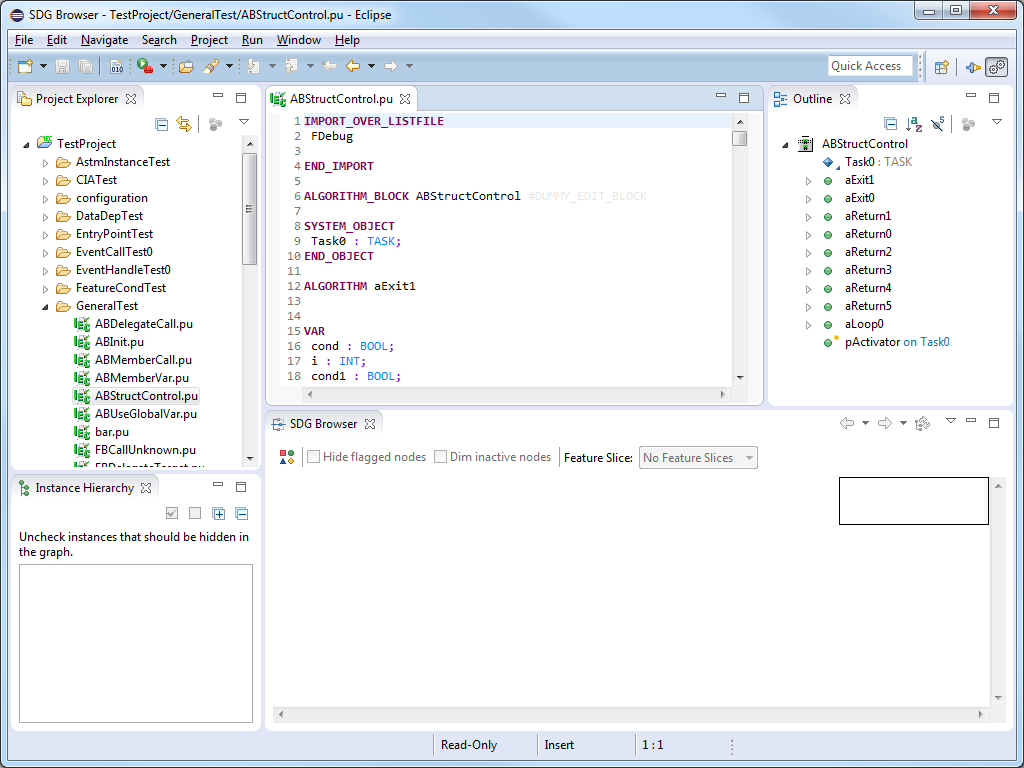
\includegraphics[width=\textwidth]{bilder/manual-editor}
  \caption{IEC file opened in Eclipse, an outline of the file is shown to the right}
  \label{fig:manual-editor}
\end{figure}


\section{Using the SDG} \label{sec:manual-sdg}

Everything shown so far works without manually building the Eclipse project, since the source code is automatically 
parsed once any of the project's files are opened. However, the SDG must be built before the \SB can be used. For large 
projects this can take several minutes.

To build the SDG, open any file within the project and then hit Ctrl+B or select \emph{Build Project} from the 
\emph{Project} menu (\autoref{fig:manual-build1}). If you try to use any of the \SB operations before the project has 
been built, you will be asked whether you want to build the project (\autoref{fig:manual-build2}).

\begin{figure}[hp]
  \centering
    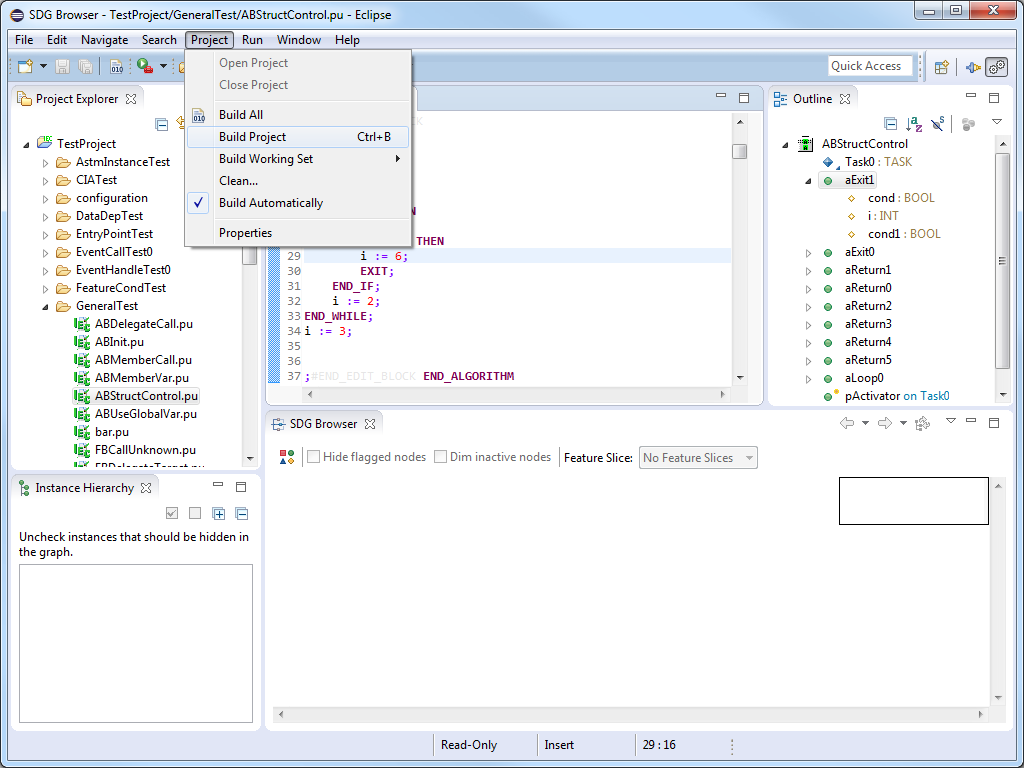
\includegraphics[width=\textwidth]{bilder/manual-build1}
  \caption{Building the IEC project before using \SB operations}
  \label{fig:manual-build1}
\end{figure}

\begin{figure}[hp]
  \centering
    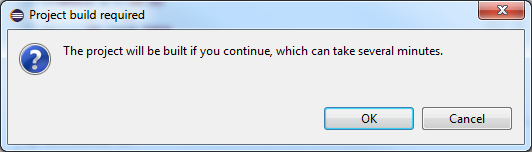
\includegraphics[scale=0.55]{bilder/manual-build2}
  \caption{Confirmation before starting a lengthy project build}
  \label{fig:manual-build2}
\end{figure}

\clearpage
The \SB operations can be accessed from the IEC editor context menu (see \autoref{fig:manual-editor_context}).

\begin{figure}[hp]
  \centering
    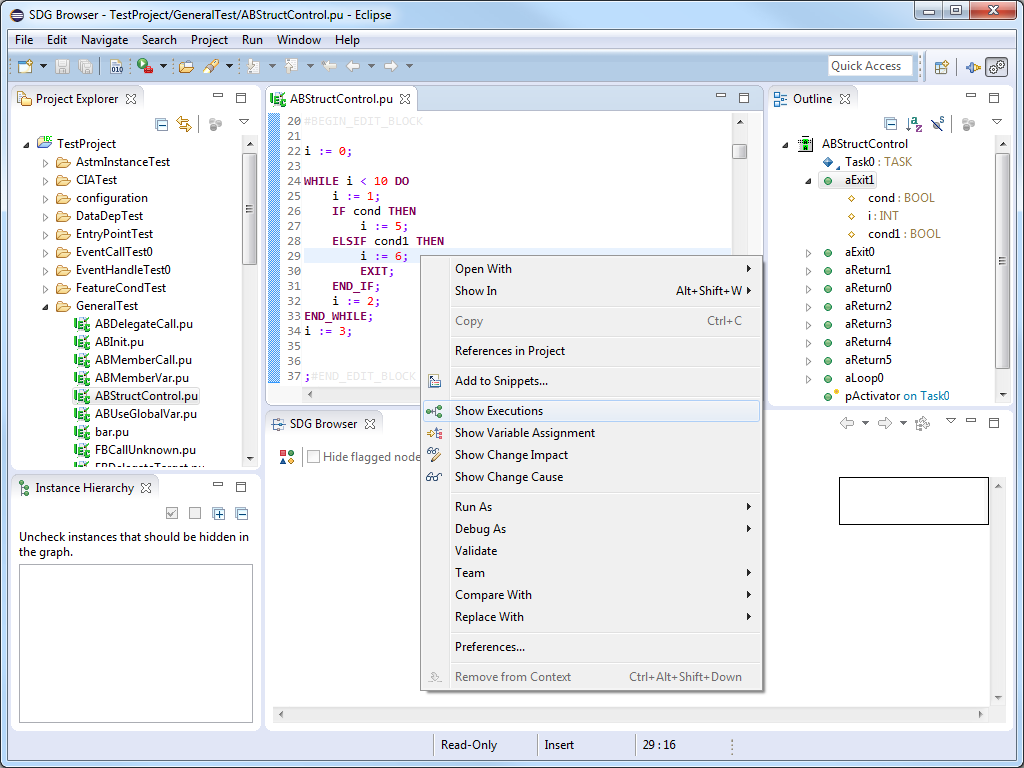
\includegraphics[width=\textwidth]{bilder/manual-editor_context}
  \caption{IEC editor context menu entries for \SB operations}
  \label{fig:manual-editor_context}
\end{figure}

\begin{figure}[hp]
  \centering
    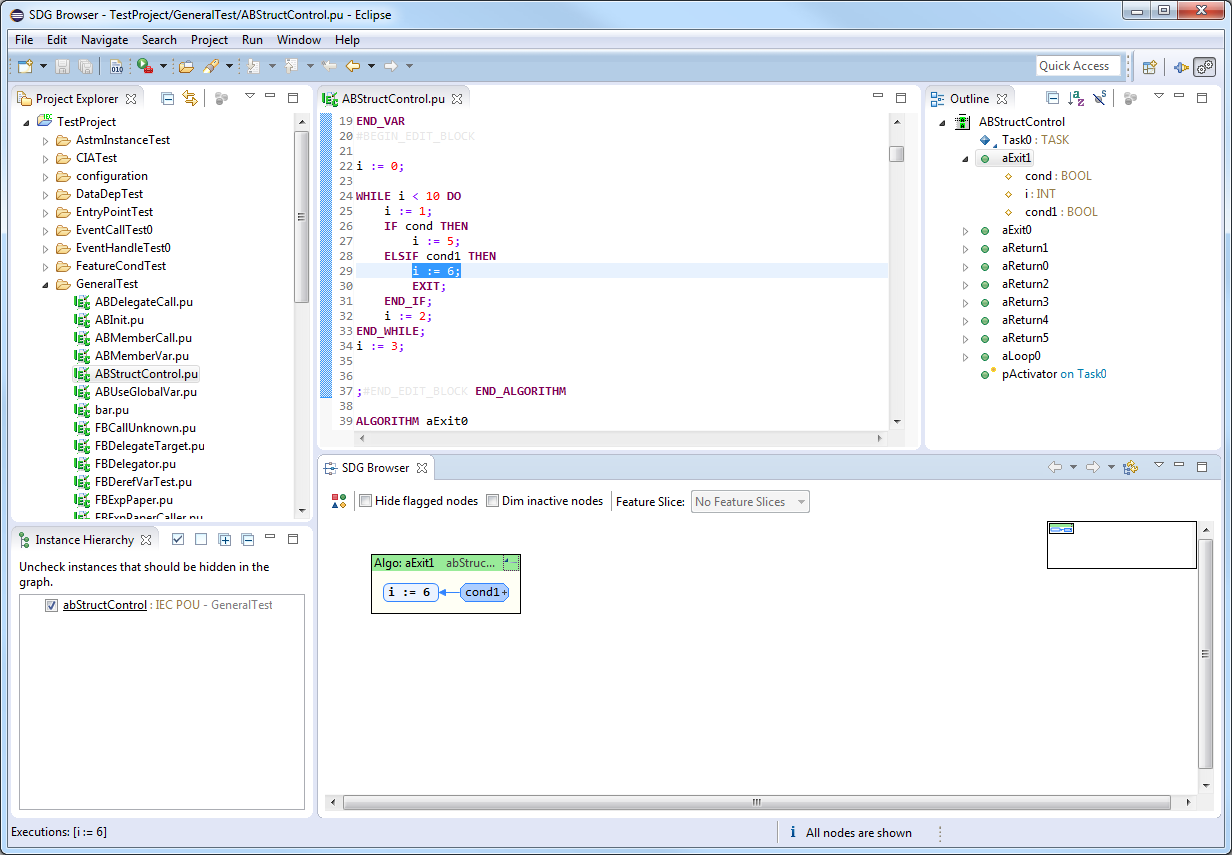
\includegraphics[width=\textwidth]{bilder/manual-executions1}
  \caption{TODO}
  \label{fig:manual-executions1}
\end{figure}

\begin{figure}[hp]
  \centering
    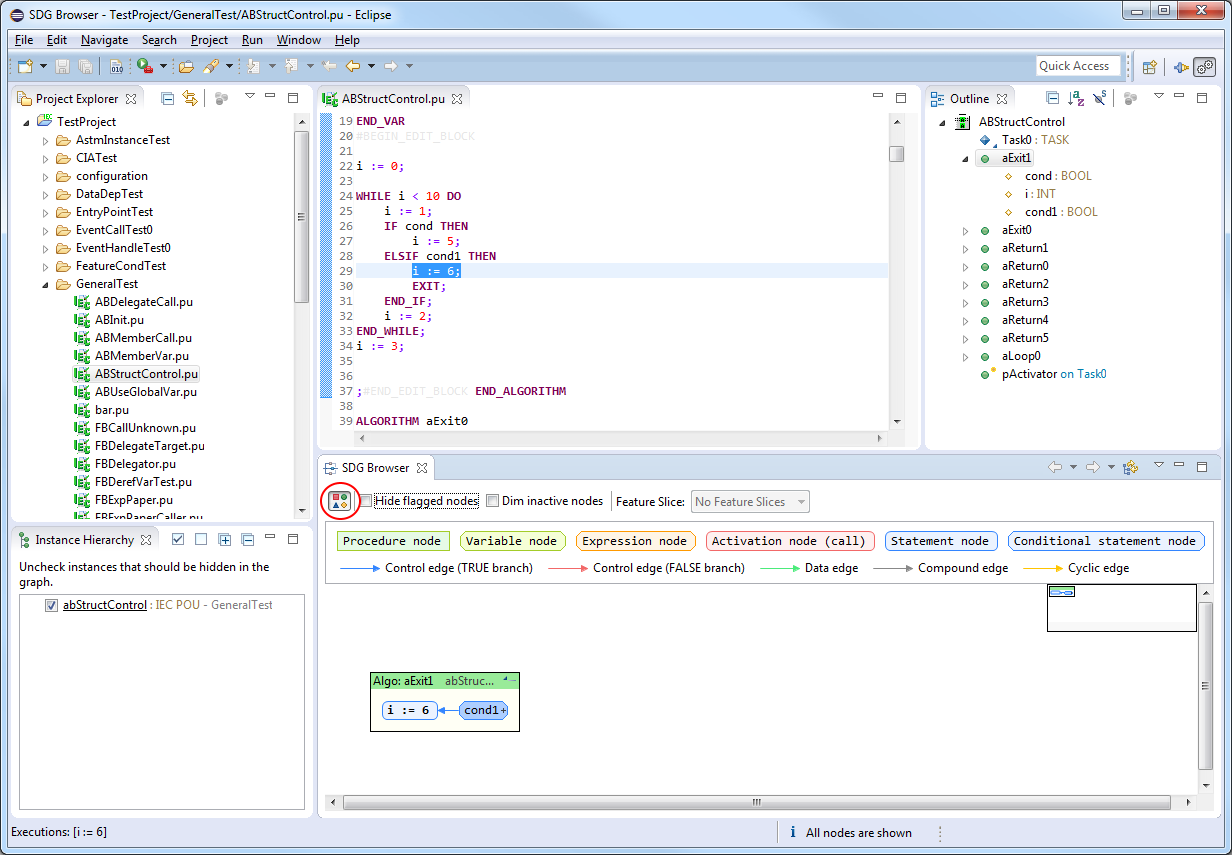
\includegraphics[width=\textwidth]{bilder/manual-legend}
  \caption{A legend shows different node and edge types}
  \label{fig:manual-legend}
\end{figure}

\begin{figure}[hp]
  \centering
    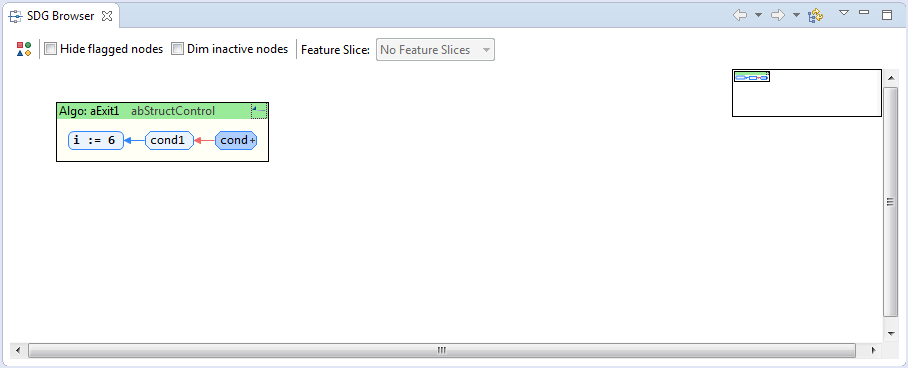
\includegraphics[width=\textwidth]{bilder/manual-executions2}
  \caption{TODO}
  \label{fig:manual-executions2}
\end{figure}

\begin{figure}[hp]
  \centering
    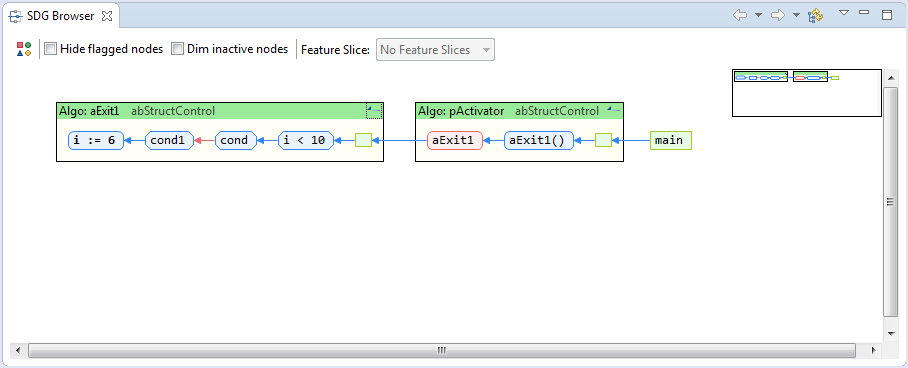
\includegraphics[width=\textwidth]{bilder/manual-executions3}
  \caption{TODO}
  \label{fig:manual-executions3}
\end{figure}


\section{Additional Features} \label{sec:manual-features}

TODO

\begin{figure}[hp]
  \centering
    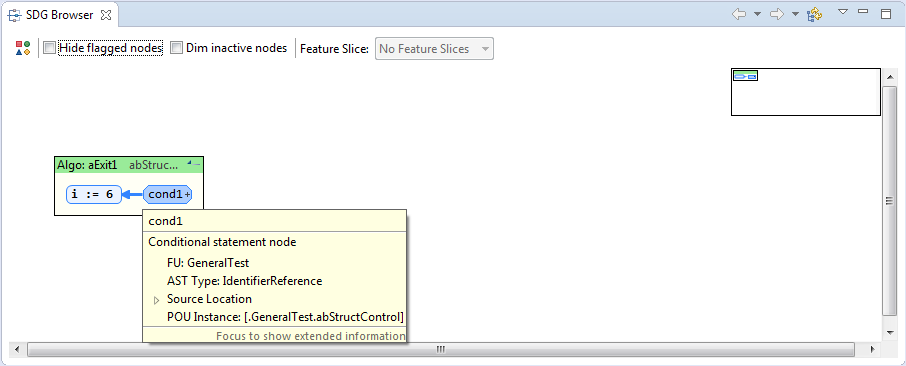
\includegraphics[width=\textwidth]{bilder/manual-tooltip}
  \caption{Tooltips provide further information about nodes and edges}
  \label{fig:manual-tooltip}
\end{figure}

\begin{figure}[hp]
  \centering
    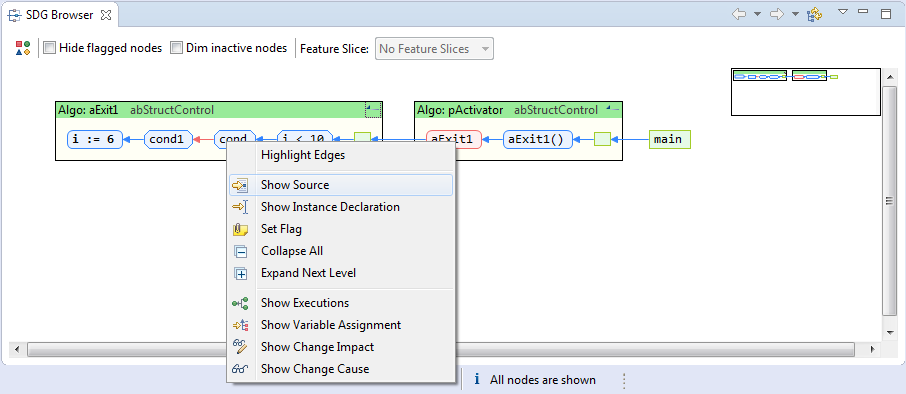
\includegraphics[width=\textwidth]{bilder/manual-node_context}
  \caption{A context menu provides additional actions on nodes}
  \label{fig:manual-node_context}
\end{figure}

\begin{figure}[hp]
  \centering
    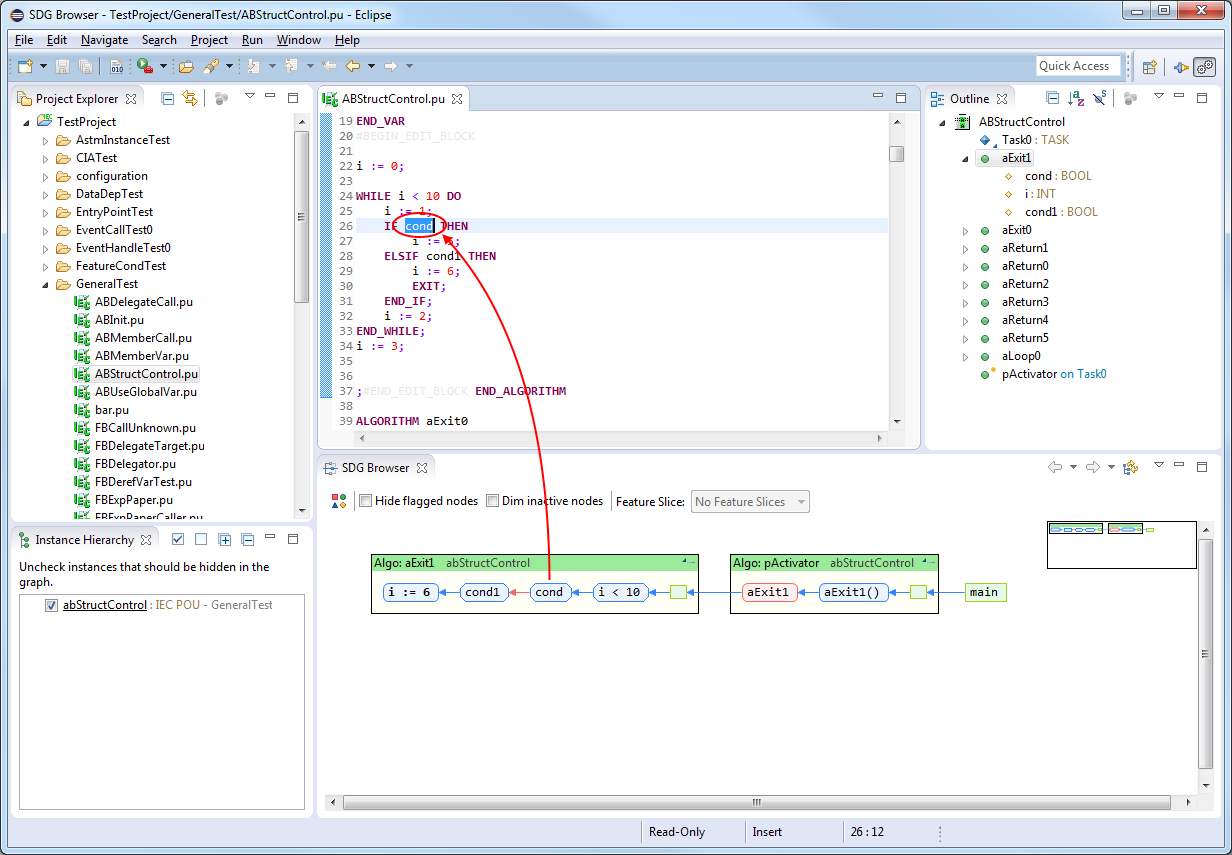
\includegraphics[width=\textwidth]{bilder/manual-show_source}
  \caption{Navigation from SDG to source code is easily accessible (Ctrl+Click on a node)}
  \label{fig:manual-show_source}
\end{figure}

\begin{figure}[hp]
  \centering
    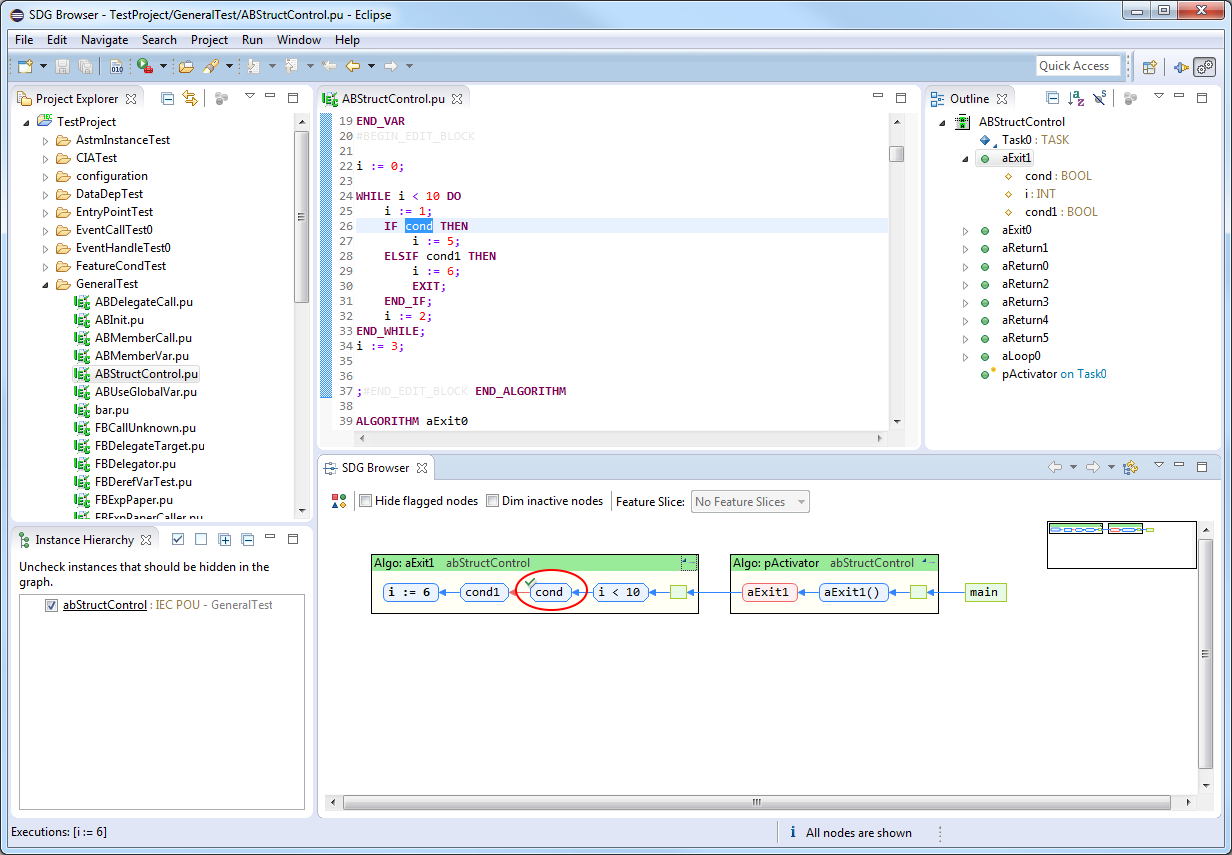
\includegraphics[width=\textwidth]{bilder/manual-flag}
  \caption{Nodes can be flagged when they have been examined}
  \label{fig:manual-flag}
\end{figure}

\begin{figure}[hp]
  \centering
    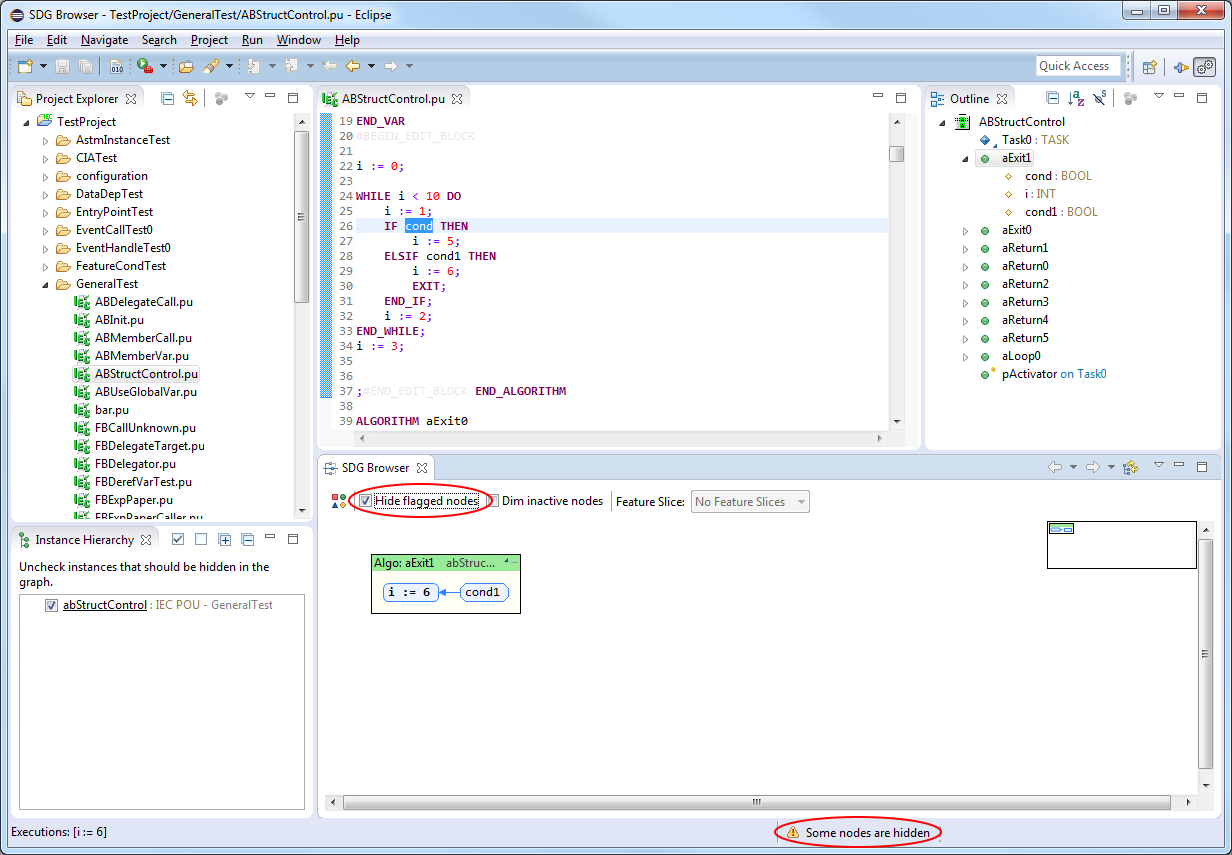
\includegraphics[width=\textwidth]{bilder/manual-hide_flagged}
  \caption{Flagged nodes can be hidden to reduce visual clutter}
  \label{fig:manual-hide_flagged}
\end{figure}


\section{Use Cases} \label{sec:manual-usecases}

TODO
